%%
%% If you intend to use figures of formats jpg, png or pdf and want the
%% output to be immediately a pdf file, compile with pdflatex.
%%
%% If you want to use eps or ps figures, your output will be a dvi
%% file that can be converted to ps and pdf formats. In this case you
%% should compile your document with latex.
%%
%%This template is compatible with both methods.
%%




\documentclass[a4paper]{IEEEtran}
\usepackage{pdfpages}
\usepackage[utf8]{inputenc}
\usepackage[T1]{fontenc}
\usepackage{graphicx}
\usepackage{amsmath}
\usepackage{amsfonts}
\usepackage{caption}
\usepackage{subcaption}
\usepackage[caption=false, ...]{subfig}

\title{{ \normalsize Master Thesis} \\
	Bluetooth Low Energy Supported Indoor Location}
\author{
	Ricardo Martins {\tt ricardo.pachecomartins@gmail.com}
	Instituto Superior T\'{e}cnico}
\date{\today}

\begin{document}
\maketitle

\begin{abstract}

	Abstract

\end{abstract}

\section{Introduction}
\label{sec:Introduction}

Indoor positioning systems have greatly evolved in the past few years due to the great success of its counter-part, the global positioning system (GPS), in outdoor environments but failure to reproduce the same results in indoor environments. Since GPS is an outdoor position systems and is based on a network of satelite, when the required scenario for position tracking is inside a building, new constraints are presented onto the process such as the attenuation and reflection of eletromagnetic waves upon collision with building walls and obstacles \cite{surveygps}. As such there was a need to find reliable indoor systems that by nature would already be able to heavily reduce the impact of some of the mentioned constraints.

In order to understand indoor position there is a need to understand the full scope of variables that come to surface when moving from outdoor to indoor. When developing a system there is a need to make sure that it can tackle the chalenges such as small space dimension which reforce the need for higher precision, a higher probability of non existent line of sight, influence of obstacles such as walls, furniture, moveable objects such as doors and human beings\cite{reviewtechniques}. All of the previously mentioned affect the way electromagnetic waves propagate in an indoor environment leading to problems related to severe multipath and reflection on existent surfaces \cite{surveywireless}. Besides propagation challenges, there are energy consumption, accuracy and deployment costs that play a critical role in deciding the viability of a proposed indoor location technique.

With the evolution of mobile devices there has been a sizeable number of different technologies that can possibly be used in indoor locationing \cite{surveywireless,survey2,survey1} such as GPS-based technologies, using high sensitivity antenas to overcome GPS's indoor issues, RFID , Wireless LAN and Bluetooth among others, allowing even for hibrid systems which make use of more than one of the technologies mentioned above. 

Another important aspect besides the chosen technology is the location detection technique which are widely varied in terms of accuracy and complexity. The simplest available category would be proximity detection which has Cell of Origin (CoO) as its most famous technique, allowing for room-based detection by assuming that the mobile target is at the cell with the strongest receiving power. This technique is widely used by system using RFID, Bluetooth and Infrared. The next category would be triangulation which uses the geometric properties of the triangle to obtain a position. The method utilized to obtain the values used in the position's calculation can be angle-based, which have implementation costs are their worst limitation; time-based, using Time-of-flight (ToF) or Round Trip Time (RTT) to obtain measures of distance from beacons; signal property based, using received signal strength indicator (RSSI) as a metric, altough it's only possible of using this metric with radio signals; dead reckoning, which calculates the actual position utilizing the last determined position and incrementing based on estimate of the device's speed.

The solution in this paper is based on the Bluetooth Low energy technology using the CoO method to obtain the device's location and as such for what technologies and location methods are concerned, only the used ones will be focused. 

In this paper is structured in a way that in \ref{sec:related} an overview of Bluetooth low energy (BLE) and existent projects and their associated architecture are presented while shedding light on the benefits and limitations of the chosen technologies, in \ref{sec:structure} the proposed system is described based on technology and method used as well as the architecture of the would system, \ref{sec:performance} analyzes the different aspects of the presented solution in terms of energetic efficiency, accuracy and response timings, finalizing in \ref{sec:future} by overviewing what could be carried out in order to further develop the existing work and by concluding the paper.


- Falta de framework, não tenho bases, vale a pena mencionar na introdução?

\section{Related Word}
\label{sec:related}

Bluetooth is a wireless technology that was created in 1994 with the objective of replacing cables connecting fixed or portable devices. At this point in time Bluetooth Special Interest Group is in charge of developing and managing this technology characterized by its robustness, low energy consuption and low cost. The Bluetooth Low Energy protocol was introduced with the Bluetooth Core Specification version 4 (also called Bluetooth Smart) circa 2010 alongside two other protocols.  Out of the three, BLE standed out for its lower power consuption, lower complexity and lower cost, while allowing for  device discovery, connection establishment and connection mechanisms. 

The BLE radio operates at the 2.4GHz band and employs a frequency hopping transceiver to combat interference and fading. It also employs two multiple access schemes: FDMA used to separate the 40 available physical channels, 37 of them are used as data channels and the remaining as advertising channels and TDMA in a polling scheme that is used when one device transmits a packet at a predetermined time and a corresponding device responds with a packet after a predetermined interval.

 \begin{figure}[htp]
	\centering
		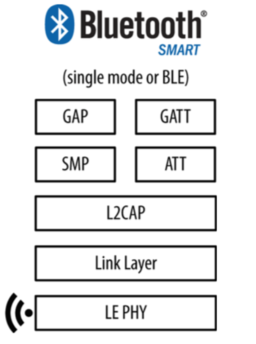
\includegraphics[width=0.5\linewidth]{figures/BLEArchitecture.png}
	\caption[Bluetooth Low Energy Architecture]{Bluetooth low energy architecture}
	\label{fig:BLEarchitecture}
\end{figure}

When looking at the BLE's architecture , which can be seen at \ref{fig:BLEarchitecture}, the Generic Access Profile (GAP) is one of the most relevant since it's responsible for working in conjunction with Generic Attribute (GATT) to define the base funcionality of BLE devices. The services that are made available by the GAP are: BLE device discovery, connection modes, security, authentication, association models and service discovery.
In addiction to this, it also defines four different roles to describe a device, allowing for the controllers to be optimized in funtion of the device's desired roles: 
Broadcaster, role optimized for transmitter-only applications; 
Observer, role optimized for receiver-only applications and it's complementary to the broadcaster role;
Peripheral, role optimized for devices that only want to suppot a single connection, allowing for a much less complex controller due to the fact that it only needs to support the slave role and not the master one; 
Central, role supports multiple connections and funtions as the initiator for all of them. These connection are all made with Peripheral devices and its controller must support the master role in a connection and allow for more complex funtions, in comparison to the remaining roles.

Another important component is the Attribute Protocol (ATT) Protocol which is responsible for implementing the Peer-to-peer(P2P) protocol between an attribute server and client. This communication happens in a dedicated fixed  channel and a server can send through it responses, notifications and indications, while the client can send requests, commands and confirmations. The ATT allows the clients to read and write values of attributes on a peer device acting as a server.

The last component is the Generic Attribute (GATT) Profile which is responsible for creating a framework for the ATT, in which it's represented the funcionalities of an ATT server. This profile describes the hierarchy of services, characteristics and attributes existent in the server and provides an interface for discovering, reading, writing and indicating service characteristics and profiles.

Bluetooth low energy devices utilize profiles which define the required functionalities of the device. It also defines application behaviour and data formats and as such when two devices comply with all the requirements of a Bluetooth profile, application interoperability is achieved. Each Bluetooth profiles describes its requirements necessary for devices to create a connection, to find available services and connection information required for making application level connections.

\begin{figure}
	\centering
		\includegraphics[width=0.5\linewidth]{figures/profile.png}
	\caption[Gatt-based profile hierarchy]{Gatt-based profile hierarchy}
	\label{fig:profile}
\end{figure}

The base profile that any Bluetooth system needs to include is the GAP. From this point, any additional profile implemented will be a superset of GAP, where GATT is included and specifies the profile hierarchy, or the structure in which profile data is exchanged. Figure  ~\ref{fig:profile} shows the hierarchy in a Gatt-based profile, with the profile being the top level and services and characteristics below. 
A profile is composed by one or more services. A service is a collection of data and associated behaviors to accomplish a particular function or feature of a device or portions of a device. A service is composed of characteristics and/or references to other services.
A Characteristic is a value that is used in a service that has properties and configuration information that descrive how the value should be accessed as well as information on how to display the value. A characteristic is defined by its declaration, its properties, its value and may also be defined by its descriptor, which describes the value or permit configuration of the server relative to the value.


When looking at what's possible to achieve using the BLE technology there is the example of Apple's creation iBeacon which was presented in 2013 with the porpuse of implementing proximity sensing systems. The device is capable of playing on the broadcaster role and as such its objective is to send nearby compatible receivers certain information. Some examples of application are to track customers or trigger location-based actions on devices such as push notifications or checking in on social media, with pratical cases such as the usage of iBeacons by McDonalds to offer special offers to their customers in their fast-food stores. An indoor location system utilizing this technology was presented by Jingjing Yang et al \cite{ibeacon}, where these devices were used to indicate a pacient of his whereabouts through the proximity sensing proprieties and this information was later transfered over to a server in order to give clients a variaty of different services, from pacient counting, to nearby department's information and offer indoor guidance to the nearest available bed. 

When utilizing BLE for indoor location the usual metric used to calculate distances is the RSSI. This metric withint the context of bluetooth brings to surface several issues such as the fact that RSSI as a metric is very accurate only when the target is within a meter of the beacon, since the value decreases as the inverse of the square of the distance to the beacon . As such when developing solutions for indoor location that require system with high accuracy capable of tracking moving objects, the usage of RSSI can't be utilized without further work. Faragher et al \cite{bleacc} tackled one of the techniques used to improve BLE system's accuracy, fingerprinting, by verifying the effects caused by the device deployment density within the required location. This experiment also puts into evidence one of the downsides of the bluetooth technology being that its scalability is low, besides requiring higher density in order to increase accuracy, due to their low range any need to increase coverage leads to increased costs.

TODO Existante work

-Cricket


-Active Bat


-Radar


-active badge


recent stuff


In 2011, LifeMap \cite{lifemap} introduced one of the first to attempt to track indoor location with unconstrained phone placement. Not Bluetooth



Zonith \cite{zonith} introduced a bluetooth based location system with the objective of tracking the position of workers in dangerous environments. Any device registered in the zonith implemented network would be continuously tracked and accounted for in each of the system's functionalities such as, sounding an alarm whenever a lone worker doesn't move or responde within a time interval (Lone worker protection) or providing a quick an precise location of any worker that has requested for help. This system's installation requires planing of the best locations to place the beacons and number required of beacons in order to be able to provide enough courage and make sure the system provides the required quality.


- BLE Projects
	

- Architecture similar stuff?


\section{Implementation}
\label{sec:struture}


The solution presented in this paper was made with the objective of presenting a generic indoor location system using bluetooth low energy. The system's architecture is presented in figure ~\ref{fig:architecture} and is divided three parts: the bluetooth low energy device, in section ~\ref{subsec:beacon} a description of the used technologies and the changes made are present;the server, whose funcionalities and stored information are described in section ~\ref{subsec:server}; and the smartphone application, whose process is described in section ~\ref{subsec:app} alongside figures that show the functional prototype. For each of these parts an explanation will be given, containing a description of each of its components specific to the presented system alongside the requirements for each to work.

\begin{figure}
	\centering
		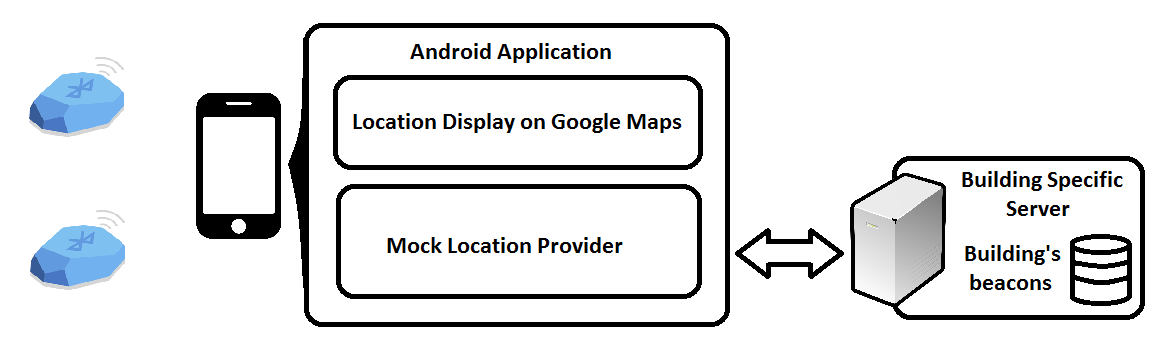
\includegraphics[width=1\linewidth]{figures/Architecture.png}
	\caption[System's Architecture]{System's Architecture}
	\label{fig:architecture}
\end{figure}

\subsection{ BLE beacon}
\label{subsec:beacon}

The beacons that were utilized are Texas Instruments CC2650STK devices which can be visualized in figure ~\ref{fig:beacon}. Alongside the device, which comes with a pre-installed bluetooth low energy program capable of giving information on each of its ten sensors through its predefined profiles, there is a texas smartphone application that can connect to a single device and read from its sensors. By using the texas Code Composer Studio (CSS), the pre-defined ble profile existant on the device could be altered. Upon further analysis of the profile, a characteristic was found for which the Universal Unique Identifier (UUID) of the service and the characteristic itself was found and as such this was the one that ended up being used to store the device's owner server's address. Since the device was already set to work as a pheripheral and it now stored the information relevant to the system, there was no need to do further work.

\begin{figure}
	\centering
		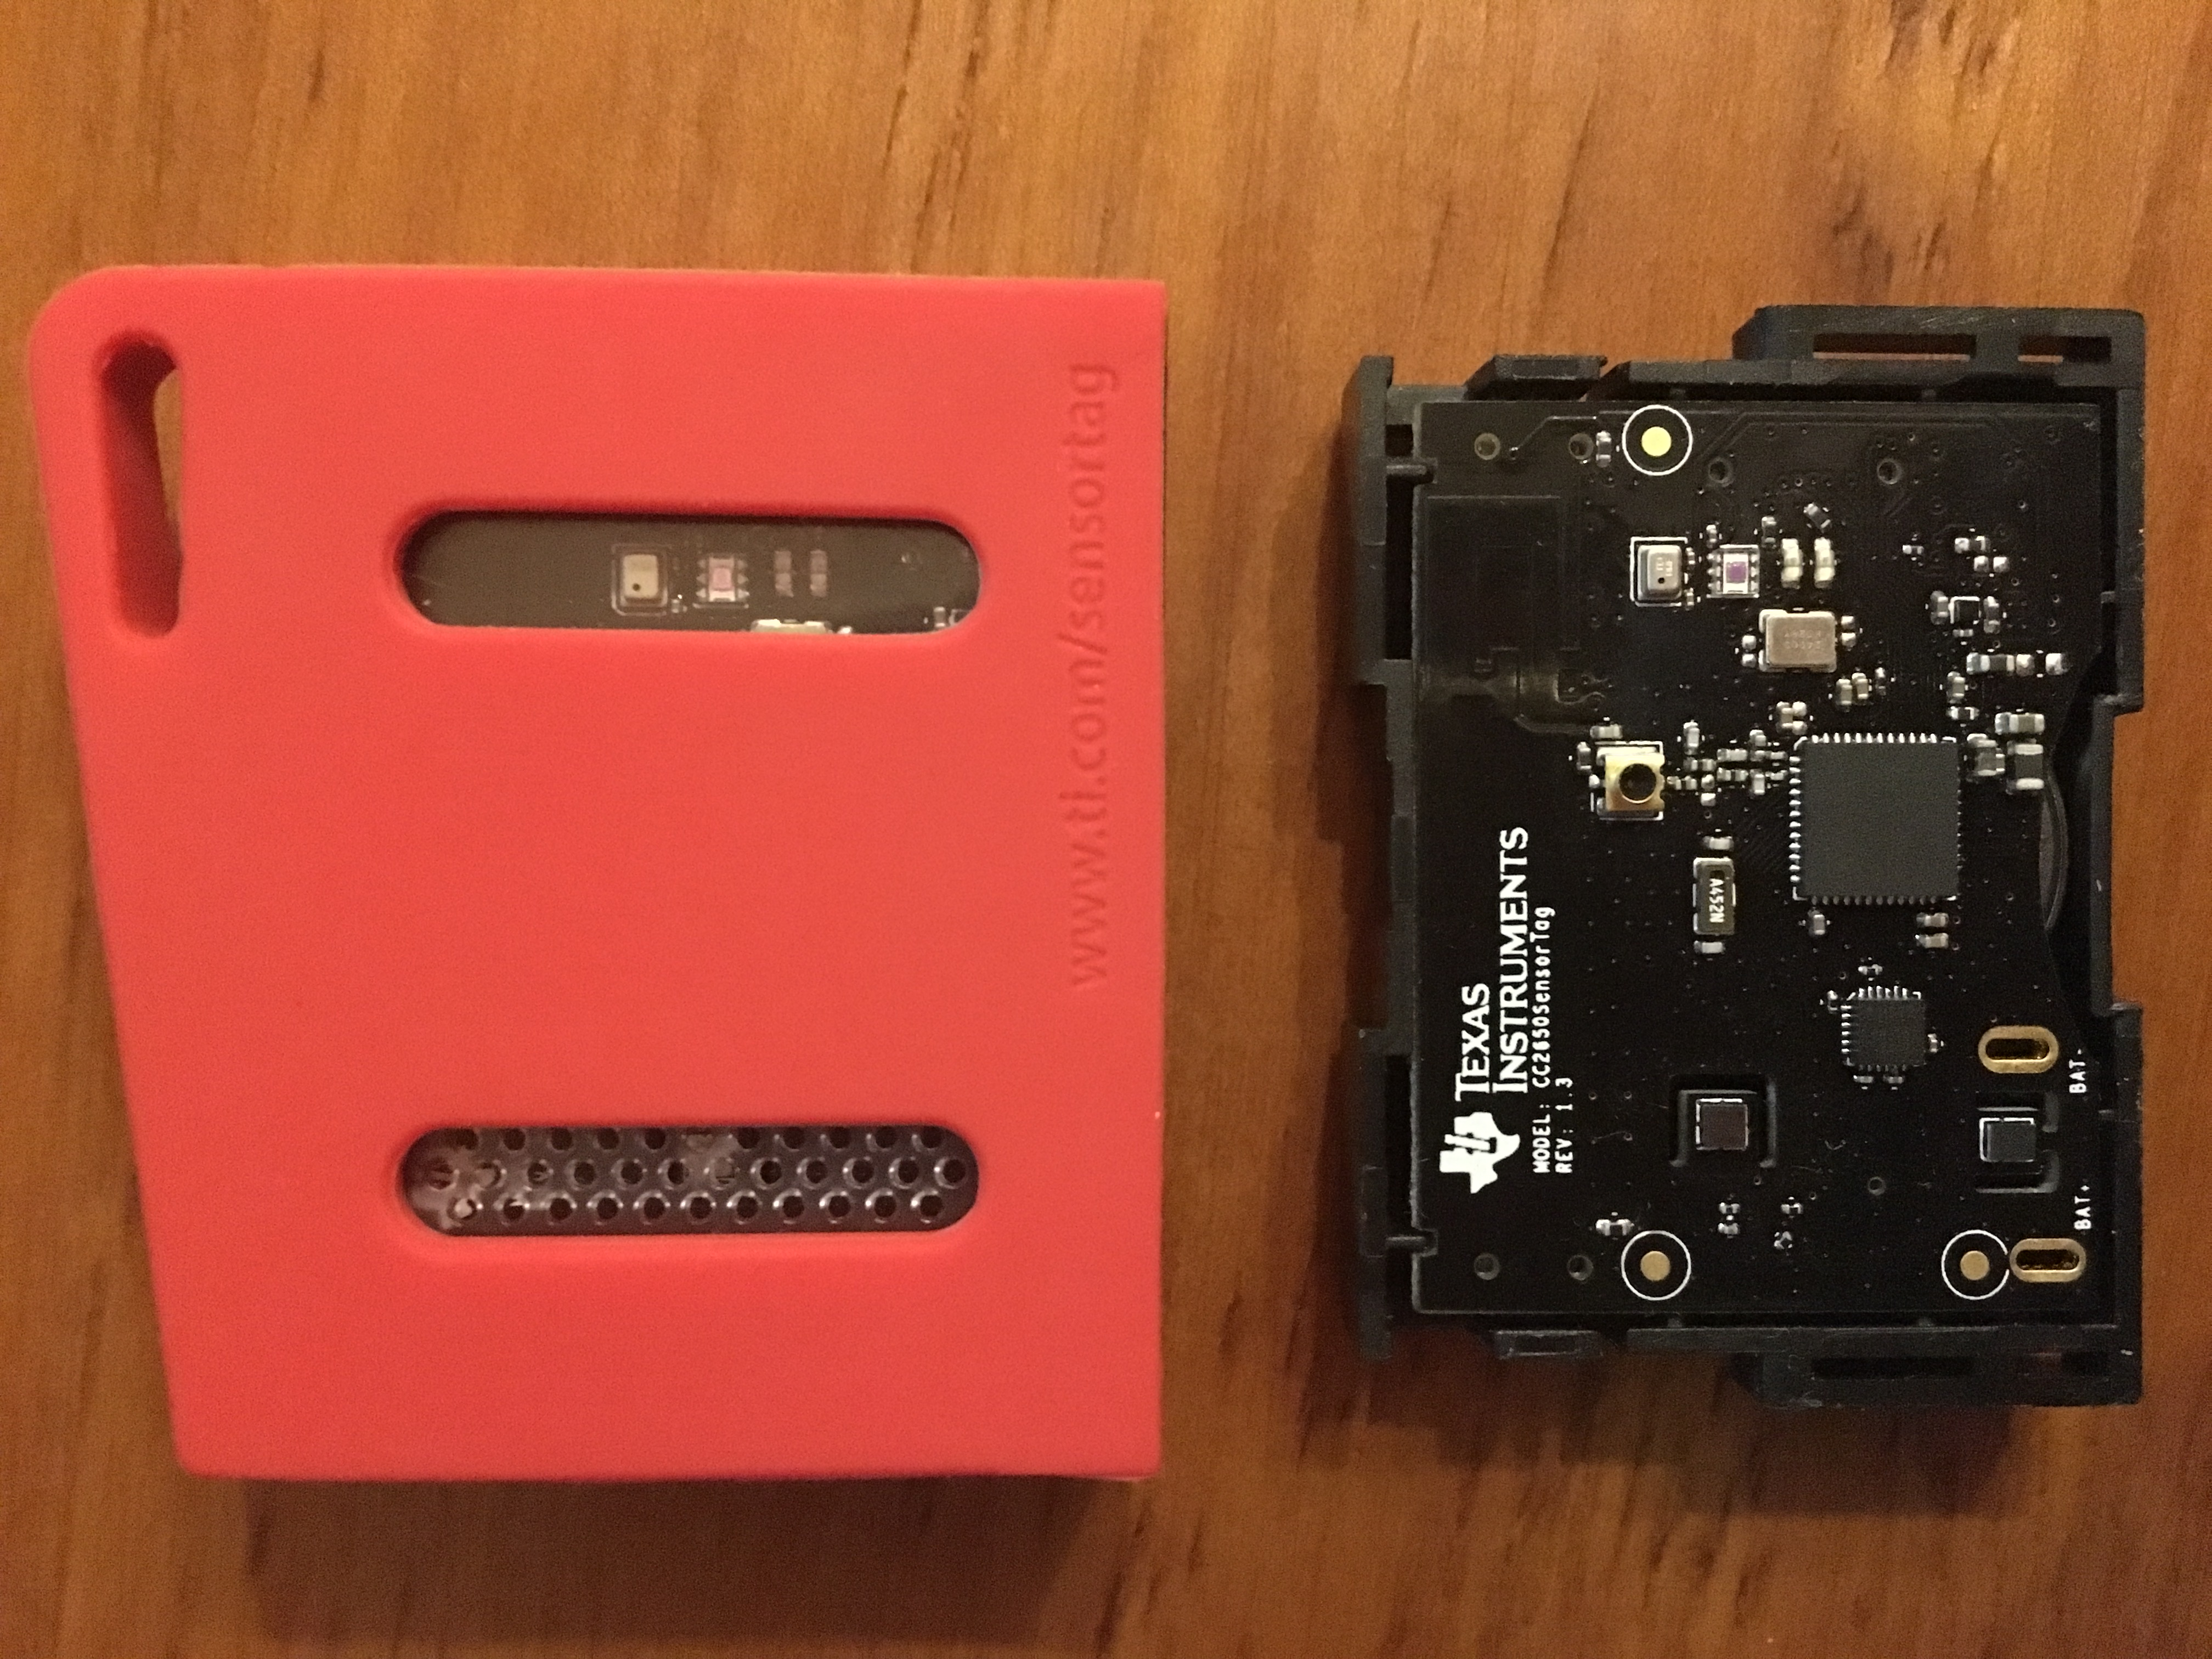
\includegraphics[width=0.5\linewidth]{figures/beacon.jpg}
	\caption[TI cc2650stk sensortag]{TI cc2650stk sensortag}
	\label{fig:beacon}
\end{figure}


\subsection{ Server}
\label{subsec:server}

The webserver was implement in Python 3 programming language. The program implements a simple tcp server capable of receiving multiple request at the same time. Each request starts with information sent from an application which include a pair of MAC address and associated RSSI value for each ble device that the same application found. Afterwards the list of pairs is filtered in order to remove any existant devices that are not present in the server's database of devices.

Each server has a database that includes only ble devices. An entry (description of a device) in this database is composed by the device's mac address, its longitude and latitude and its building, floor and room name. In addition to the database, a server when initiated can store additional location info such as the server's street, number, zipcode, city and country, allowing this information to be transmited to the client in order to offer an additional level of location description to the user. The whole location specific information can be visualised in figure ~\ref{fig:AppMenu}.

Upon having filtered the initial list of pairs, the Cell of Origin (CoO) technique is applied by verifying which of the devices produced a stronger signal on the receptor. Upon obtaining the closest device an answer is sent to the application containing all of the information associated to the server and the selected device.


- Describe the Database ( insert image example of database with a few entries?? )

- Mention capability to Insert aditional info, at the moment it displays geocoding on pop up menu in figure ~\ref{fig:AppMenu}.



\subsection{ Application}
\label{subsec:app}

The Smartphone application was developed for Android using the Android Studio IDE. The Application is divided in two primary functional blocks, the Mock location Provider and the Google Maps Integrated Display, as can be visualized in figure ~\ref{fig:Architecture}.

The Mock Location Provider is implemenented as if it was a Location provider, such as gps. The application functions works as a listener to a Location provider, in this case it listens to the Mock Provider that was implemented. By implementing the whole process of obtaining a location inside a service (the mock provider) , a new level of abstraction is added to the application. As such, whenever the application is signaled to obtain the user's current location, a request is made to the associated location provider and the application only need to listen for the answer that eventualy arrives.

\begin{figure}
	\centering
		\includegraphics[width=0.5\linewidth]{figures/RequestLocation.png}
	\caption[Mock Location Provider Workflow]{Mock Location Provider Workflow}
	\label{fig:MockProvider}
\end{figure}

The Mock Location Provider incorporates the first three steps present in figure ~\ref{fig:MockProvider}, which will now be explored individualy. The first step indicates the gathering of information of the surroundings of the user's device. When a request is made to the provider, a scan for nearby bluetooth low energy devices is made which will put the smartphone in a state of listening for incoming ble advertisement packets for half a second ( NEED TO VERIFY VALUE AND JUSTIFY, THERE WAS A PAPER ON THIS TODO). During this scanning period, each time a device is found, the advertisement is registered in a list, which have a duplication prevention mechanism implemented. Once the period is over, the provider has avaliable a list of all the ble devices within range.   

The second step involves taking the created list of devices, obtain a server adress and forward the same list to it. Once the first step is completed, the provider will analyze each entry at a time. For each device the provider will attempt to respond to the caught advertisement packet, resulting in a created connection.  Once the connection is created the provider asks for the available services of the paired device. Upon receiving an answer, the list of services is swoop while looking for the service with the wanted UUID. If the device doesn't have the UUID that the provider is looking for, it can assume that the paired ble is not a beacon of our system, as such the connection is terminated. When the provider identifies that the device has the system's UUID, it requests the device to provide the service's existant characteristics. The provider will receive a list composed of the service's characteristics and it will search in it for the system's characteristics UUID, the one which contains the device's server's address. This search has the objective of confirming that the service existant in this device is indeed the one that was implemented for the system and not a device with another service that happened to have the same UUID. For any service outside those that are documented in the Bluetooth Special Interest Group (SIG), who have a specific UUID attached to them, the UUID is generated randomly and as such there is a small chance of collision. Once the wanted characteristic is found, the provider requests the device to read its value and stores the received value in a list. This list will contain the servers of the devices that were found, and for each address there will be a list corresponding to each device , and their corresponding rssi values, from the same owner. In order to quicken the previously described process, the provider keeps in cache the most recent contacted devices. Before attempting a connection, the provider confirms that the device isn't found in cache and when finishing a process, the associated device is inserted into the cache.

When every device has been contacted, a voting system is actioned which will decide from the list of servers which one it will send the collected information to. The voting system uses an exponential function in order to attribute a weight to each server. INSERT FUNCTION AND EXPLAINATION.

The voting system was implemented with the objective providing a thin security layer by allowing multiple devices of the same server to overcome a single attacker's device which happened to be close to the user. After obtaining each server's values, the one with the highest value is chosen and sent the list with all the devices. 

The Third step involves a simple client/server tcp interaction. The application starts off by formulating the message that it will later on send to the server, this message includes all pairs of device mac address and its associated rssi value captured by the application on the first step. Once the message is computed, the application attemps to create a connection with the server at the chosen address at the end of step two. With the connection established, the message is forwarded to the server and the application is put onto blocked state where it awaits for an answer. Upon arrival, the answer received is checked for valid location, its information is process and the connection is terminated. The information contained inside the received message, which was described in section ~\ref{subsec:server}, is then processed into the adequate class capable of storing a geographic location and the same is broadcasted from the mock location provider to its listener. 



One of the current limitations of the android API that deals with BLE is that the interface on the smartphone that is used to connect with a device has a fixed timeout time.  MIGHT JUST NEED TO BE IMPROVED TODO


The Google Maps Integrated display is implemented using the Google Maps Android API. By using Google Maps it was possible to aliviate the weight on application since there wasn't need implement file transfer of indoor building's maps from each dedicated server to each request, which aliviated the servers aswell since there was no need to store its associated building's maps on it. Managing the maps was something that was aswell fortunately unnecessary and as such all these features were provided by google maps service. By making this development choice, the system as whole became closer to the desired generic approach while making possible for seamless transition between indoor/outdoor maps. The only imposed restriction is related to the addiction of new indoor maps onto the google maps, which is possible and well documented but dependent on a third party.

The Fourth step is called when the application receives a proper location from the request made onto the location provider. With the device's location known, a marker is placed on the map with the obtain coordinates (longitude, latitude), the camera is moved in order to be centralized on the position and fully displaying the indoor level map, and the menu visible on figure ~\ref{AppMenu} is updated with the information that is bundled with the received location. In order to show the correct level on a multi level building, the "floor" information present in the menu is utilized. The API allows for obtaining a list of existant levels on which the maps' camera is focused and as such it's possible to find out to which level the provided locaiton belongs and make so that the application shows it.

The pop-up menu was implemented to demonstrate the capacity of providing additional information associated with each location, be it geo-location taxonomy as it is currently implemented or possibly a description of the located room, an hyperlink of some sort or any other type of data that someone implemented this system would like to provide to its users.  

The final state of the implemented system can be visualized in figure ~\ref{fig:AppFocus} and figure ~\ref{fig:AppMenu}. The first displays the case of obtaining a location, where the marker has been placed and the camera zoomed

\begin{figure}
	\centering
		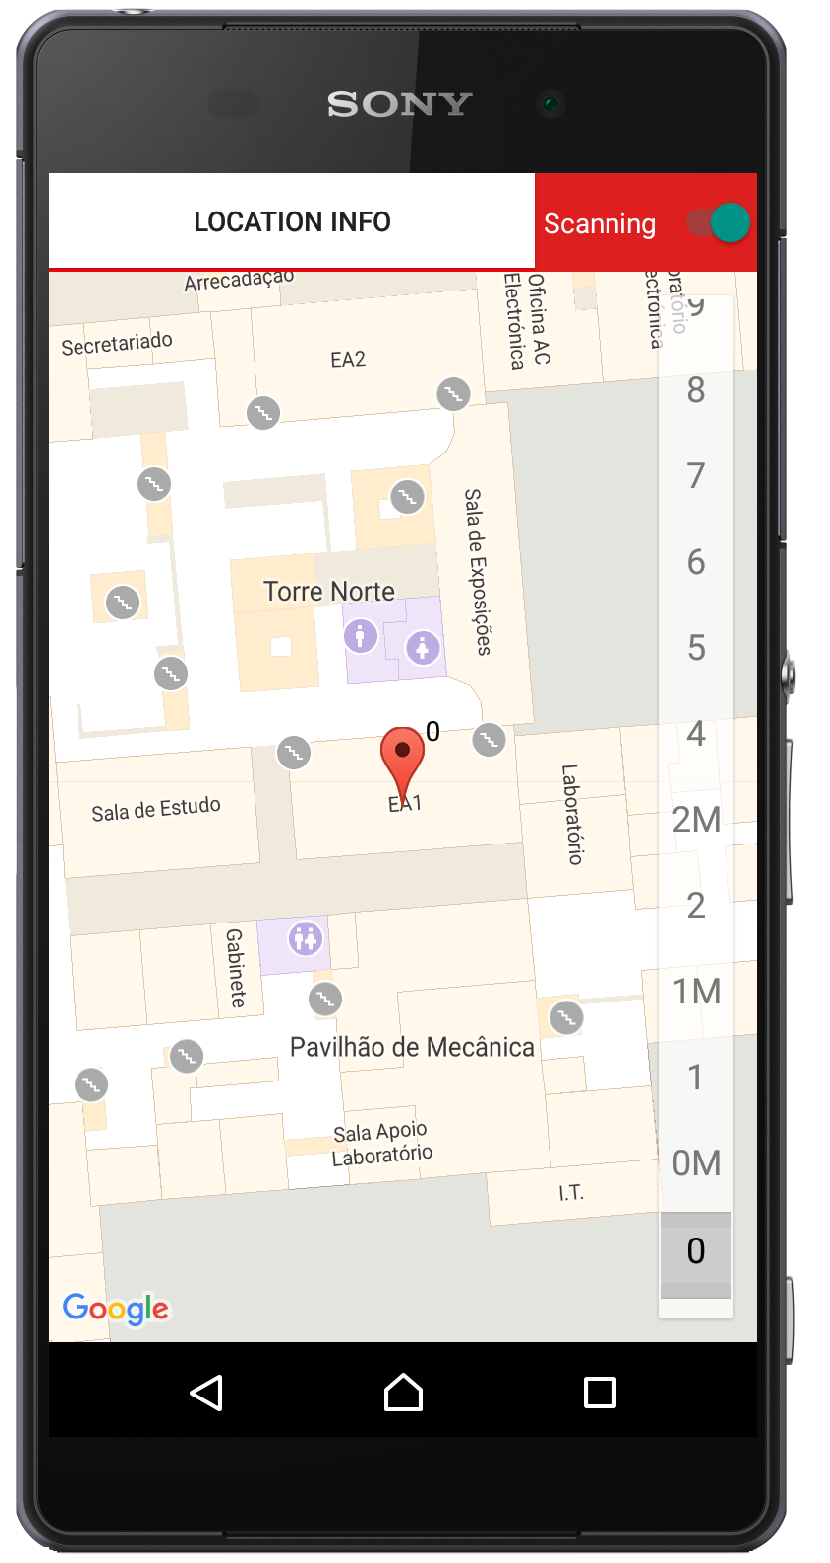
\includegraphics[width=0.5\linewidth]{figures/app_focused.png}
	\caption[Application screen showing a focused location on a room]{Application screen showing a focused location on a room}
	\label{fig:AppFocus}
\end{figure}

\begin{figure}
	\centering
		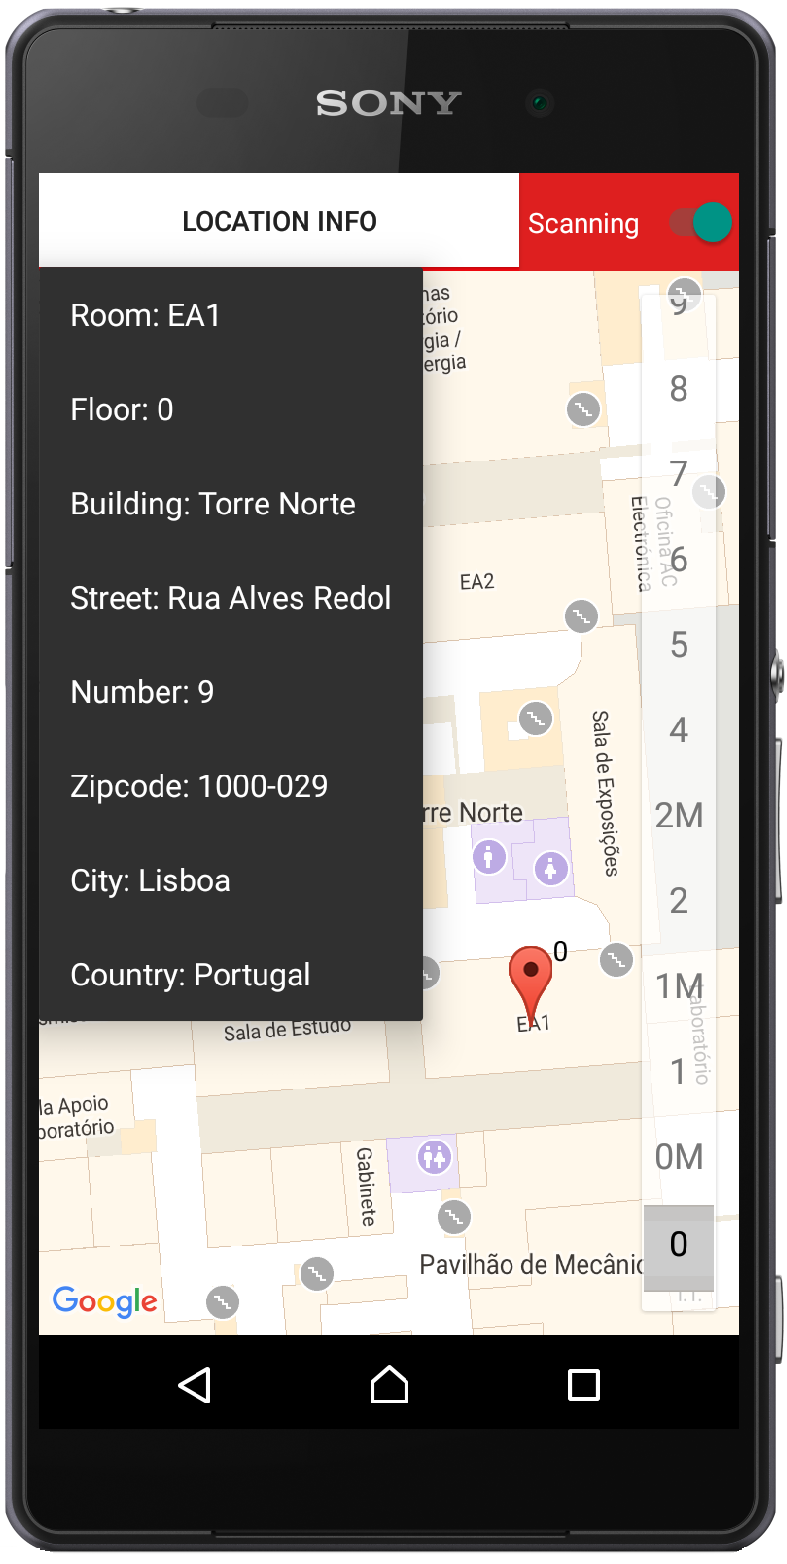
\includegraphics[width=0.5\linewidth]{figures/app_focused_menu.png}
	\caption[Application screen showing additional information of location]{Application screen showing additional information of location}
	\label{fig:AppMenu}
\end{figure}






\section{Performance Analysis}
\label{sec:performance}

- Energy Consumption in general

- Energy consumption vs Cycle time vs Accuracy?

- Location Accuracy

- Time for request completion

- Data Requiremnts?
 



\section{Future Work}
\label{sec:future}

- Possible Improvement: Paralel ble connections; Improvements on lateration algorithm;  Rest depends on the Performance results

- Conclusions




\begin{thebibliography}{9}

\bibitem{surveygps}
 \texttt{Hakan Koyuncu, Shuang Hua Yang ;A Survey of Indoor Positioning and Object Locating Systems http://paper.ijcsns.org/07_book/201005/20100518.pdf}

\bibitem{surveywireless}
 \texttt{Hui Liu; Survey of Wireless Indoor Positioning Techniques and Systems http://www.pitt.edu/~dtipper/2011/Survey1.pdf} 

\bibitem{reviewtechniques}
 \texttt{Zahid Farid, Rosdiadee Nordin, and Mahamod Ismail; Recent Advances in Wireless Indoor Localization Techniques and System}

\bibitem{survey2}
 \texttt{Hakan Koyuncu, Shuang Hua Yang; A Survey of Indoor Positioning and Object Locating Systems; http://paper.ijcsns.org/07_book/201005/20100518.pdf}

\bibitem{survey1}
 \texttt{Jiang Xiao, Zimu Zhou,Youwen Yi and Lionel M. Ni; A Survey on Wireless Indoor Localization from the Device Perspective; http://www.tik.ee.ethz.ch/~zzhou/paper/csur16-xiao.pdf}

\bibitem{blecore}
\texttt{ }

\bibitem{ibeacon}
\texttt{ Jingjing Yang, Zhihui Wang and Xiao Zhang ;An iBeacon-based Indoor Positioning Systems for Hospitals; http://www.sersc.org/journals/IJSH/vol9_no7_2015/16.pdf}

\bibitem{bleacc}
\texttt{ R. Faragher and R. Harle; An Analysis of the Accuracy of Bluetooth Low Energy for Indoor Positioning Applications; http://www.cl.cam.ac.uk/~rmf25/papers/BLE.pdf}

\bibitem{lifemap}
\texttt{Yohan Chon and Hojung Cha; LifeMap: A SmartphoneBased Context Provider for Location-Based Services; https://pdfs.semanticscholar.org/cb50/e7344494f8b8fdfeba160f814cbfe3ce3356.pdf}

\bibitem{zonith}
\texttt{http://media.teldio.com/pdfs/Teldio_Indoor}

 
 
\end{thebibliography}

\end{document}
